
%(BEGIN_QUESTION)
% Copyright 2011, Tony R. Kuphaldt, released under the Creative Commons Attribution License (v 1.0)
% This means you may do almost anything with this work of mine, so long as you give me proper credit

In this process, a single ``shutdown controller'' device sends actuating signals to two redundant block valves, actuating them simultaneously.  The purpose of this system is to provide a very high level of assurance that the process line will shut off when needed:

$$\includegraphics[width=15.5cm]{i03793x01.eps}$$

The figure given for each block valve in the above diagram is the {\it mean time between failure} (MTBF) for that valve, from the perspective of the valve sticking open and failing to shut when called to do so.

\vskip 10pt

Calculate the probability of this block valve system failing to shut off flow in the line, assuming both valves are absolutely brand-new, and already burned-in by the manufacturer.

\vskip 10pt

Next, calculate the probability of this block valve system failing to shut off flow in the line after 5 years of continuous operation.

\underbar{file i03793}
%(END_QUESTION)





%(BEGIN_ANSWER)

PFD (brand-new) = 0

\vskip 10pt

PFD (5 yr) = 0.0217702

%(END_ANSWER)





%(BEGIN_NOTES)

At $t$ = 0, the reliability (R) for each block valve is 100\%, and so there is no probability of failure on demand (PFD = 0).

\vskip 10pt

After 5 years, the reliability of each valve drops off accordingly:

$$R = e ^{- t \over MTBF}$$

$$R = e ^{- {5 \over 35}} = 0.86688$$

$$R = e ^{- {5 \over 28}} = 0.836464$$

This means the PFD for each valve (probability of {\it not} functioning as designed) will be 0.133122 and 0.163536, respectively.

\vskip 10pt

The PFD for the whole system is the probability that the first valve {\it and} the second valve will both fail.  This is equal to 0.0217702.

%INDEX% Safety, system reliability: Mean Time Between Failures (MTBF)
%INDEX% Safety, system reliability: probability of failure on demand (PFD)

%(END_NOTES)


